%%%% utfpr-slides.tex, 2019/12/01
%%%% Copyright (C) 2015-2019 Luiz E. M. Lima (luizeduardomlima@gmail.com)
%%
%% This work may be distributed and/or modified under the conditions of the
%% LaTeX Project Public License, either version 1.3 of this license or (at your
%% option) any later version.
%% The latest version of this license is in
%%   http://www.latex-project.org/lppl.txt
%% and version 1.3 or later is part of all distributions of LaTeX version
%% 2005/12/01 or later.
%%
%% This work has the LPPL maintenance status `maintained'.
%%
%% The Current Maintainer of this work is Luiz E. M. Lima.
%%
%% This work consists of the files utfpr-slides.sty and utfpr-slides.tex.
%%
%% A brief description of this work is in readme.txt.

%% Detecção e aviso sobre comandos obsoletos
% \RequirePackage[l2tabu, orthodox]{nag}

%% Classe de documento e opções
%%%% Modo apresentação: descomente o comando \documentclass[]{beamer}
\documentclass[%% Opções: [*] comente para remover; [>] passada para pacotes
  10pt,%% Tamanho de fonte: 10pt, 11pt, 12pt, etc.
  aspectratio = 43,%% Razão de aspecto: 169 (16:9), 43 (4:3), etc.
  compress,%% Redução de tamanho das barras de navegação [*]
  % handout,%% Versão que usa especificações de sobreposição do folheto [*]
  t,%% Alinhamento vertical dos quadros: b (fundo), c (centro) e t (topo)
  english,%% Idioma secundário (penúltimo) [>]
  brazilian,%% Idioma primário (último) [>]
]{beamer}
%%%% Modo artigo: descomente o comando \documentclass[]{article}
% \documentclass[%% Opções: [>] passada para pacotes
  % a4paper,%% Tamanho de papel: a4paper, letterpaper, etc.
  % english,%% Idioma secundário (penúltimo) [>]
  % brazilian,%% Idioma primário (último) [>]
% ]{article}

%% Pacotes utilizados
\usepackage[%% Opções:
  Times   = false,%% Fontes Times (roman) e Arial (sans serif): true ou false
  BibURLs = false,%% Links de URLs nas referências: true ou false
  GovLogo = false,%% Logomarca do Governo Federal: true ou false
  MECLogo = false,%% Logomarca do Ministério da Educação: true ou false
  LogosOn = false,%% Logomarcas nos títulos dos slides: true ou false
  ABNTNum = none,%% Estilo numérico ABNT: none (AUTOR, ANO), dflt (1) e brkt [1]
]{utfpr-slides}

\usepackage{siunitx}
\usepackage{listings}
\usepackage{color}
\usepackage[super]{nth}
\usepackage{datetime}
\beamertemplatenavigationsymbolsempty
\iflanguage{english}{%
  \newdateformat{myformat}{\monthname[\THEMONTH]  \nth{\THEDAY}, \THEYEAR}
}{
\newdateformat{myformat}{\THEDAY de \monthname[\THEMONTH] de \THEYEAR}
}
\definecolor{mylilas}{RGB}{170,55,241}
\lstset{language=Matlab,%
	basicstyle=\footnotesize\ttfamily,breaklines=true,%
	morekeywords={matlab2tikz},
	keywordstyle=\color{blue},%
	morekeywords=[2]{1}, keywordstyle=[2]{\color{black}},
	%morekeywords={laplace,ilaplace},
	deletekeywords={roots,residue,poly,polyder},
	identifierstyle=\color{black},%
	stringstyle=\color{mylilas},
	commentstyle=\color{black!50!green},%
	upquote=true,
	showstringspaces=false,%without this there will be a symbol in the places where there is a space
	%    numbers=left,%
	%    numberstyle={\tiny \color{black}},% size of the numbers
	%    numbersep=9pt, % this defines how far the numbers are from the text
	%emph=[1]{for,end,break},emphstyle=[1]\color{red}, %some words to emphasise
	%emph=[2]{word1,word2}, emphstyle=[2]{style},    
}
%% Arquivo de referências
\addbibresource{utfpr-slides.bib}

%% Arquivos de logomarcas (diretório ``Logos''): comente para remover
%\logoevent{evento}%% Logomarca do evento
%\logoorg{evento-org}%% Logomarca da organização promotora
%\logoextinst{inst-ext}%% Logomarca da instituição do autor externo
\logoprog{ppgse-ct}%% Logomarca do programa ou do curso
\logodept{ppgse-ct}%% Logomarca do departamento ou da coordenação
\logoextra{ppgse-ct}%% Logomarca extra (à esquerda da logomarca do câmpus)
\logocampus{utfpr-ct}%% Logomarca do câmpus

%% Informações do documento
%%%% Título: [CURTO]; {LONGO}
\title[Sistema de Localização Híbrida por AoA e MLT]{%
  \bfseries%
  Estimativa de localização de alvos em ambientes internos por meio de fusão de algoritmos de Multilateração e Ângulo de Chegada.
}
%%%% Subtítulo
\subtitle{%
  Dissertação de Mestrado
}
%%%% Assunto
\subject{Nome e/ou Sigla do Congresso, Seminário ou Evento Técnico/Científico}
%%%% Congresso, seminário ou evento técnico/científico:
%%%% descomente os comandos \author[]{}, institute[]{} e \titlegraphic{}
%%%%%% Autor(es): [CURTO]; {LONGO}%
%\author[P. M. Autor(a) et al.]{%
%  Andrey Fabris\inst{1}%
%  \athanks[0009-0003-9107-6261]{andreyfabris@alunos.utfpr.edu.br}{%
%    Programa de Pós-Graduação em Sistemas de Energia%
%  }%
%}
%%%%%% Instituição(ões) e e-mail(s): [CURTO]; {LONGO}
%\institute[UTFPR]{%
%  \affil[1,3,5]{\utfprname, Curitiba, Paraná, Brasil}%
%  \and\email[1]{andreyfabris@alunos.utfpr.edu.br}%
%}
%%%%%% Logomarcas do evento
\titlegraphic{\eventlogos}
%%%% Defesa de trabalho acadêmico:
%%%% descomente os comandos \author[]{}, institute[]{} e \titlegraphic{}
%%%%%% Autor(a): [CURTO]; {LONGO}
\author[A. Fabris.]{%
  Andrey Fabris\inst{1}%
  \athanks[0009-0003-9107-6261]{andreyfabris@alunos.utfpr.edu.br}{%
    Programa de Pós-Graduação em Sistemas de Energia%
  }%
}
%%%%%% Instituição: [CURTO]; {LONGO}
 \institute[UTFPR-CT/PPGSE]{%
  \affil{%
     \utfprname%
     \and Câmpus Curitiba (CT)%
     \and Programa de Pós-Graduação em Sistema de Energia (PPGSE)%
   }%
   \and\email{andreyfabris@alunos.utfpr.edu.br}%
   \and Orientador: Prof. Dr. Ohara Kerusauskas Rayel%
   \and Coorientador: Prof. Dr. João Luiz Rebelatto
 }
%%%%%% Logomarcas da instituição
% \titlegraphic{\institutelogos}
%%%% Câmpus: {SIGLA}; {NOME}
\campus{CT}{Campus Curitiba}
%%%% Departamento, coordenação, programa ou curso: [LOGO]; {SIGLA}; {NOME}
\departament[ppgse-ct]{PPGSE}{Programa de Pós-Graduação em Sistemas de Energia}
%%%% Data: [CURTO]; {LONGO}
\date[\myformat\today]{\myformat\today}

%% Início do documento
\begin{document}

\mode<presentation>{%% Modo apresentação: página de título e sumário
  \frame{\titlepage}%
%   \frame[allowframebreaks]{%
%     \frametitle{\contentsname}%
%     \framesubtitle{~}%
%     \tableofcontents%
%   }%
}

\mode<article>{\maketitle}%% Modo artigo: página de título
%%%%%%%%%%%%%%%%%%%%%%%%%%%%INTRODUÇÃO###########################################################
\section{Introdução}\label{sec:intro}
%%%%%%%%%%%%%%%%%%%%%%%%%%%%TEMA###########################################################
\subsection{Tema}\label{ssec:tema}

\begin{frame}
%%%%%TEXTO
O tema \textit{IoT} apareceu nos anos 2000 e se tornou uma parte importante na indústria e também na vidas das pessoas em poucas décadas \cite{Farahsari2022}. A Figura \ref{fig:crescimento_iot} mostra o crescimento desses dispositivo ao longo dos anos e sua previsão atpe o ano de 2023.

\begin{figure}[!htb]
\centering%
\caption{Crescimento de dispositivos inteligentes, em bilhões.}%
\mode<presentation>{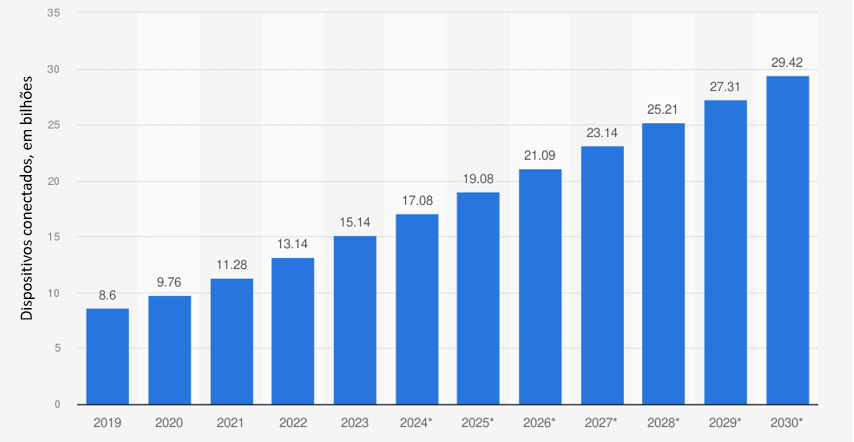
\includegraphics[width = 0.6\columnwidth]{Figuras/crescimento_iot.png}}
\source{adaptado de \textcite{Vailshery2023}.}
\label{fig:crescimento_iot}
\end{figure}
\end{frame}
%%%%%%%%%%%%%%%%%%%%%%%%%%%%OBJETIVOS###########################################################
\subsection{Objetivos}\label{ssec:objetivos}
\begin{frame}
\begin{block}<+->{Objetivos Gerais}
\begin{itemize}
\item Estudar e implementar modelos de estimativa de localização.
\item Aplicar filtros estocásticos para obtenção de estimativas.
\item Propor modelo de estimativa por meio de fusão de algoritmos.
\end{itemize}
\end{block}
\end{frame}
%%%%%%%%%%%%%%%%%%%%%%%%%%%%PROCEDIMENTOS###########################################################
\subsection{Procedimentos Metodológicos}\label{ssec:procedimento}
\begin{frame}
%%%%%TEXTO
\end{frame}

%%%%%%%%%%%%%%%%%%%%%%%%%%%%JUSTIFICATIVA###########################################################
\subsection{Justificativa}\label{ssec:justificativa}
\begin{frame}
%%%%%TEXTO
\end{frame}



\section{Revisão Bibliográfica}\label{sec:revisao}
%%%%%%%%%%%%%%%%%%%%%%%%%%%%TEMA###########################################################
\subsection{Modelos de localização}\label{ssec:modelos}

\begin{frame}
A Tabela \ref{tab:resumo_tecnicas} mostras as comparações de algumas técnicas para estimativa de localização.

    \begin{table}[!htb]
    	\centering
        \mode<presentation>{\scriptsize}%% Modo apresentação: tamanho de fonte
    	\caption{Comparação de técnias de estimativas de localização.}
    	\label{tab:resumo_tecnicas}
    	\begin{tabular*}{\columnwidth}{@{\extracolsep{\fill}}|llll|}
    		\hline
    		Técnica & Tecnologia & Acurácia & Processamento \\
            \hline
    		\hline
    		  Tempo de Chegada  & Banda Ultralarga & Dezenas de centímetros & Médio \\
            RSSI  & \textit{Bluetooth} & Alguns metros & Baixo \\
            Ângulo de Chegada   & \textit{Bluetooth} & Até poucos metros & Alto \\
            \textit{Round Trip Time}  & Banda Ultralarga & Alguns centímetro & Médio \\
    		\hline
    	\end{tabular*}
    	\source{adaptado de \cite{Farahsari2022}.}
    \end{table}
\end{frame}


\subsection{Filtragem estocástica}\label{ssec:filtragem}

\begin{frame}
O Filtro de Kalman é composto por dois passos principais: predição e atualização. 
\begin{block}<+->{Predição}
\begin{align}
\hat{\mathbf{x}}_{k} &= \mathbf{A}\hat{\mathbf{x}}_{k-1} + \mathbf{G}\mathbf{u}_{k-1},\label{KF_begin}\\
	\mathbf{P}_{k} &= \mathbf{A}\mathbf{P}_{k-1}\mathbf{A}^{T}+\mathbf{Q}.
\end{align}
\end{block}
\begin{block}<+->{Atualização}
\begin{align}
	\mathbf{K}_{k} &= \mathbf{P}_{k}\mathbf{C}^{T}(\mathbf{C}\mathbf{P}_{k}\mathbf{C}^{T}+\mathbf{R}_{k})^{-1}, \\
	\hat{\mathbf{x}}_{k} &= \hat{\mathbf{x}}_{k}+\mathbf{K}_{k}(\mathbf{z}_{k}-\mathbf{C}\hat{\mathbf{x}}_{k}), \\
	\mathbf{P}_{k} &= (\mathbf{I} - \mathbf{K}_{k}\mathbf{C})\mathbf{P}_{k}(\mathbf{I} - \mathbf{K}_{k}\mathbf{C})^{T}+\mathbf{K}_{k}\mathbf{R}_{k}\mathbf{K}_{k}^{T}.\label{KF_end}
\end{align}
\end{block}
\end{frame}


%%%%%%%%%%%%%%%%%%%%%%%RESULTADOS###########################################################
\section{Resultados}\label{sec:revisao}
%%%%%%%%%%%%%%%%%%%%%%%%%%%%TEMA###########################################################
\subsection{}\label{ssec:modelos}

\begin{frame}
%%%%%TEXTO
\end{frame}


%%%%%%%%%%%%%%%%%%%%%%%CONCLUSÕES###########################################################
\section{Conclusões}\label{sec:revisao}
%%%%%%%%%%%%%%%%%%%%%%%%%%%%TEMA###########################################################
\subsection{}\label{ssec:modelos}

\begin{frame}
%%%%%TEXTO
\end{frame}

%%%%%%%%%%%%%%%%%%%%%%%PRÓXIMOS PASSOS###########################################################
\section{Próximos Passos}\label{sec:revisao}
%%%%%%%%%%%%%%%%%%%%%%%%%%%%TEMA###########################################################
\subsection{}\label{ssec:modelos}

%%%%%%%%%%%%%%%%%%%%%%%PRÓXIMOS PASSOS###########################################################
\section{Cronograma}\label{sec:revisao}
%%%%%%%%%%%%%%%%%%%%%%%%%%%%CRONOGRAMA###########################################################
\subsection{}\label{ssec:modelos}

\begin{frame}
%%%%%TEXTO
\end{frame}




\mode<presentation>{%% Modo apresentação: referências
  \section{\refname}\label{sec:refs}%
  \frame[allowframebreaks]{%
    \framesubtitle{~}%
    \printbibliography[heading = none]%
  }%
}

\mode<article>{\printbibliography}%% Modo artigo: referências

\section{Agradecimentos}\label{sec:agrad}

\respnotice[Declaração de Responsabilidade]{O autor é o único responsável pelas informações contidas neste documento.}

\begin{frame}{}{\mode<presentation>{~}}
\mode<presentation>{%% Modo apresentação: agradecimentos e declaração de responsabilidade
  Aos presentes, pela atenção\sfootnote[frame]{\faStickyNoteO~\textbf{\respnoticetitle:}\space\MakeLowercase{\respnoticetext}}.%
}
\end{frame}

\mode<article>{%% Modo artigo: declaração de responsabilidade
  \section{\respnoticetitle}\label{sec:declar}%
  \respnoticetext%
}

%% Fim do documento
\end{document}
